%==============================================================================
% AgentForge --- Overleaf-ready paper scaffold
% Compiles out-of-the-box on Overleaf (pdfLaTeX). Zero uploaded style files:
% IEEEtran.cls and IEEEtran.bst ship with TeX Live / Overleaf.
%
% Build order on Overleaf: pdfLaTeX -> BibTeX -> pdfLaTeX -> pdfLaTeX
% To switch to a single-column "report" look, change the documentclass to
%   \documentclass[11pt]{article}  and delete the IEEEtran-specific commands.
%==============================================================================
\documentclass[conference]{IEEEtran}

\usepackage[T1]{fontenc}
\usepackage[utf8]{inputenc}
\usepackage{lmodern}
\usepackage{graphicx}
\usepackage{booktabs}
\usepackage{amsmath}
\usepackage{url}
\usepackage[hidelinks]{hyperref}   % load last

\graphicspath{{figures/}}

% A compact verbatim-style block for the API listing.
\newcommand{\code}[1]{\texttt{#1}}

\begin{document}

\title{AgentForge: A Self-Improving Selection Layer\\ for Agentic Workflows}

\author{%
  \IEEEauthorblockN{Minseok Kim}
  \IEEEauthorblockA{Stanford University \\
  \texttt{dkim27@stanford.edu}}
}

\maketitle

\begin{abstract}
Production LLM agents typically hardcode \emph{how} they act on each task: a
developer picks one multi-step workflow---one prompting strategy, tool-use
pattern, or decomposition---freezes it, and hand-edits prompts when it
underperforms. We argue that workflow \emph{selection} should itself be learned
online. We present \textbf{AgentForge}, a domain-agnostic selection layer that
treats per-task workflow choice as a multi-armed bandit: given a small set of
candidate workflows (arms) and any cheap reward signal, an online policy learns
which workflow wins on which tasks, concentrates selection there, and persists
what it learns across runs. AgentForge ships as a ten-line SDK over a ladder of
policies---$\epsilon$-greedy, UCB1, Thompson sampling, a contextual LinUCB
bandit, and a multi-step REINFORCE controller. On the BIRD-SQL text-to-SQL
benchmark with \code{gpt-4o-mini}, the bandit learns online to avoid a harmful
decomposition workflow and reaches a cumulative reward of $22.3$ over $60$
episodes---above a random baseline ($20.3$) and approaching a post-hoc oracle
($27.0$). The \emph{same} selector learns the best strategy across three further
domains (code generation, agentic search, context compaction), and the
contextual and multi-step rungs improve per-task and trajectory-level selection.
We report honest negative results: when two workflows are statistically tied,
the selector's value is \emph{surfacing} the tie, not manufacturing a winner.
\end{abstract}

\begin{IEEEkeywords}
LLM agents, multi-armed bandits, online learning, workflow selection, text-to-SQL.
\end{IEEEkeywords}

%------------------------------------------------------------------------------
\section{Introduction}
%------------------------------------------------------------------------------
LLM agents are stochastic, and different tasks reward different \emph{strategies}.
For text-to-SQL, an easy question may need a single prompt; a wide schema may need
exploration first; a nested question may need decomposition. In practice a developer
guesses one workflow per use case and freezes it. When it underperforms, a human
reads traces and hand-edits prompts---indefinitely. The result is a standing tax:
you overpay by running a heavy workflow everywhere, or underperform by running the
cheap one, and you never \emph{know} which is best. Evaluation and tracing tools tell
you the agent is broken; none of them \emph{fix} the choice.

The agent stack has recently commoditized \emph{orchestration}: Google ADK, the
OpenAI Agents SDK, Microsoft's Agent Framework, LangGraph, and CrewAI all make it
easy to \emph{write} how an agent acts. The missing layer is \emph{learning which
strategy to actually run}. That is the gap AgentForge targets.

\textbf{Contribution.} We contribute a \emph{learned policy at the
workflow-selection layer} of an agent system---a layer where selection is
ordinarily hardcoded or heuristic. Three framing points keep the claim precise:

\begin{itemize}
  \item \textbf{Selector, not a self-rewriting agent.} The policy makes \emph{one
  discrete selection decision per task}; it does not modify workflow internals.
  \item \textbf{Bandit, not (full) RL.} Selection is a one-step decision with no
  sequential credit assignment. We add a multi-step REINFORCE rung only for an
  explicit trajectory-control environment (Sec.~\ref{sec:ladder}).
  \item \textbf{Composition-novel, not algorithm-novel.} $\epsilon$-greedy is
  textbook; the novelty is a learned selector over \emph{multi-step workflow
  compositions}. The closest commercial analogs are LLM routers (RouteLLM, Not
  Diamond, Martian), which swap a single \emph{model}; we select among multi-step
  \emph{workflows}.
\end{itemize}

Concretely, AgentForge is (i) a reusable, domain-agnostic kernel,
\code{WorkflowSelector}, that takes any set of \code{task}$\rightarrow$\code{output}
callables plus a \code{(task, output)}$\rightarrow[0,1]$ reward; and (ii) a
text-to-SQL case study on BIRD-SQL that grounds the kernel in a real,
execution-based reward. We additionally demonstrate the kernel across code, search,
and compaction domains, and climb a policy ladder from $\epsilon$-greedy to a
contextual bandit and a multi-step controller.

\begin{figure*}[t]
  \centering
  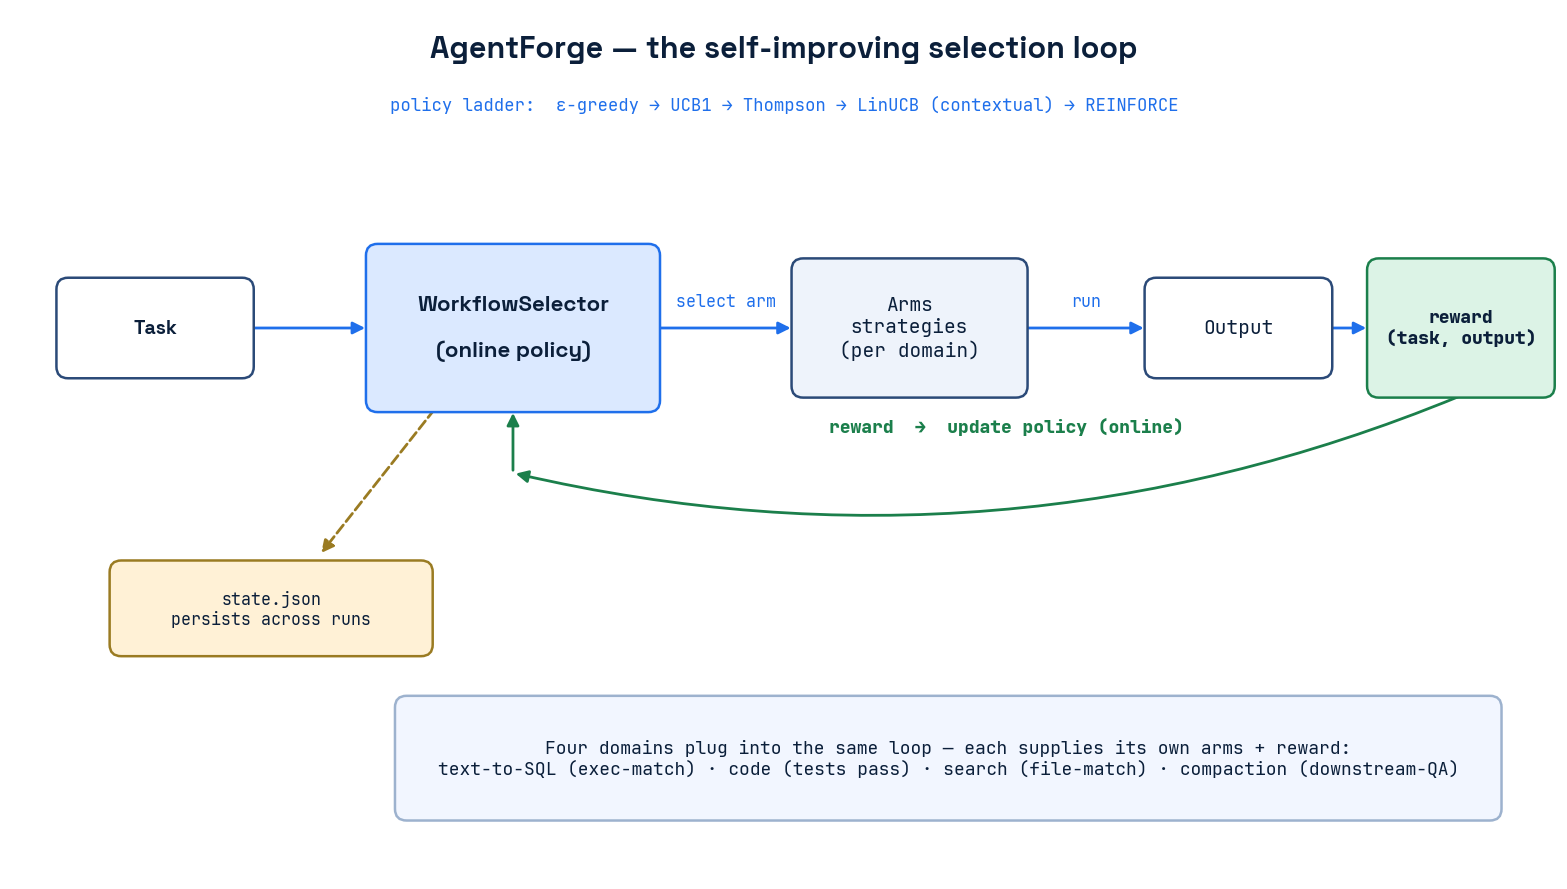
\includegraphics[width=0.92\textwidth]{architecture.png}
  \caption{AgentForge architecture. A task enters; the \code{WorkflowSelector}'s
  policy picks a strategy (arm); the strategy runs (one or more LLM calls); a reward
  function scores the output; the policy updates \emph{online} and \emph{persists} to
  disk. Each domain plugs its own arms $+$ reward into the same loop, and the policy
  is swappable along the ladder $\epsilon$-greedy $\rightarrow$ UCB1 $\rightarrow$
  Thompson $\rightarrow$ contextual LinUCB $\rightarrow$ multi-step REINFORCE.}
  \label{fig:arch}
\end{figure*}

%------------------------------------------------------------------------------
\section{Related Work}
%------------------------------------------------------------------------------
\textbf{Text-to-SQL workflows.} DIN-SQL~\cite{dinsql} and DAIL-SQL~\cite{dailsql}
show that decomposition and in-context strategy materially change accuracy on
Spider and BIRD~\cite{bird}; they fix one pipeline. AgentForge instead treats such
pipelines as interchangeable arms and \emph{learns} which to use online.

\textbf{Bandits and contextual bandits.} We build on classical online learning:
$\epsilon$-greedy and UCB1~\cite{ucb1}, Thompson sampling~\cite{thompson}, and
LinUCB~\cite{linucb} for contextual selection. Our contribution is not a new
algorithm but their application as a \emph{selection layer over multi-step LLM
workflows}, with persistence across runs.

\textbf{Model routers.} RouteLLM~\cite{routellm} and commercial routers (Not
Diamond, Martian) learn to dispatch a query to one of several \emph{models}, usually
offline from preference data. AgentForge selects among multi-step \emph{workflows}
or tool-use patterns---not a single model---and learns online from the user's own
reward.

\textbf{Workflow optimization and agent self-improvement.} DSPy~\cite{dspy} and
AFlow~\cite{aflow} optimize or search the \emph{internals} of one program offline;
Voyager~\cite{voyager}, Reflexion~\cite{reflexion}, and Self-Refine~\cite{selfrefine}
improve a single agent's behavior through memory or self-critique. These are
complementary: one can offline-optimize each arm with DSPy, then let AgentForge
select among the optimized arms online. The closest relative learns to compose
agentic workflows with a cost-aware reward but does so offline with a frozen policy;
AgentForge is, in one line, ``that idea, but online, persistent, and packaged.''

%------------------------------------------------------------------------------
\section{Method}
%------------------------------------------------------------------------------
\subsection{Workflow selection as a bandit}
A task $x$ arrives from a stream. The agent has $K$ fixed workflows
$\{a_1,\dots,a_K\}$, each a callable $a_k: x \mapsto y$ that may issue several LLM
calls internally. A policy $\pi$ selects an arm $a_k$; the workflow produces an
output $y$; a reward function $r(x,y)\in[0,1]$ scores it. The policy updates its
estimate of arm value and the loop repeats. For the non-contextual rungs we estimate
$\hat{Q}(a_k)$ as the running mean reward of arm $k$ and select with probability
$1-\epsilon$ the $\arg\max_k \hat{Q}(a_k)$, else a uniform random arm
($\epsilon=0.1$). This is one discrete decision per task: there is no intra-workflow
credit assignment.

\subsection{The \code{WorkflowSelector} kernel}
The reusable product is a domain-agnostic kernel: bring your own arms and reward.

\begin{figure}[t]
\centering
\fbox{\begin{minipage}{0.93\columnwidth}
\small\ttfamily
from agentforge import WorkflowSelector\\[2pt]
selector = WorkflowSelector(\\
\hspace*{1em}arms=\{"fast": fast\_fn,\\
\hspace*{3.2em}"careful": careful\_fn,\\
\hspace*{3.2em}"use\_tools": tool\_fn\},\\
\hspace*{1em}reward=lambda t, o: 1.0 if ok(o) else 0.0,\\
\hspace*{1em}policy="epsilon-greedy",\quad\# or ucb1, ...\\
\hspace*{1em}persist="state.json",\quad\# learns across runs\\
)\\
result = selector.run(task)\quad\# pick$\rightarrow$run$\rightarrow$score$\rightarrow$update
\end{minipage}}
\caption{The ten-line drop-in. Each arm is any \code{task}$\rightarrow$\code{output}
callable (a prompt variant, a tool-use pattern, a different model, or a whole
multi-step workflow); the reward is any signal the caller already has (tests
passing, an eval score, a thumbs-up, execution match).}
\label{fig:api}
\end{figure}

\subsection{The policy ladder}
\label{sec:ladder}
The same kernel exposes a ladder of policies via a single \code{policy=} argument:

\begin{itemize}
  \item \textbf{$\epsilon$-greedy / UCB1 / Thompson} learn the best arm \emph{on
  average} across the task stream.
  \item \textbf{LinUCB (contextual)} featurizes each task $x$ into $\phi(x)$ and
  learns a per-task policy, selecting
  $\arg\max_k\, \theta_k^\top\phi(x) + \alpha\sqrt{\phi(x)^\top A_k^{-1}\phi(x)}$,
  so it can pick \emph{different} arms for different tasks.
  \item \textbf{REINFORCE (multi-step)}~\cite{williams} targets a genuine sequential setting---an
  ``iterate-or-stop'' environment in which the controller decides, at each hop,
  whether to refine or to halt---trained with reward-to-go and a running-mean
  baseline. This is the one rung that is full policy-gradient RL rather than a
  bandit.
\end{itemize}

\subsection{The text-to-SQL instantiation}
Our real-reward case study instantiates three arms behind one interface
(\code{run(task, llm)}$\rightarrow$\code{WorkflowResult}), so the bandit treats them
as interchangeable actions:
\textbf{(0) direct}---a single LLM call mapping schema $+$ question to SQL;
\textbf{(1) schema\_explore}---identify the relevant tables, then write SQL against
that subset; and
\textbf{(2) decompose}---split into sub-questions, solve each, and compose the final
query. The reward is \emph{binary execution match}: we execute the candidate SQL and
the gold SQL against the task's SQLite database and assign reward $1$ if the result
sets match (order-insensitive unless the query has \code{ORDER BY}), else $0$;
errors and timeouts score $0$. This is execution accuracy, not string match.

%------------------------------------------------------------------------------
\section{Experimental Setup}
%------------------------------------------------------------------------------
We run on the BIRD-SQL~\cite{bird} development set across four databases
(\textit{california\_schools}, \textit{financial}, \textit{formula\_1},
\textit{superhero}), drawing a difficulty- and database-balanced pool spanning all
three BIRD difficulty levels. The model is \code{openai/gpt-4o-mini} served via
OpenRouter at temperature $0$. The mid-tier model is deliberate: a frontier model
solves nearly everything and collapses the selection signal, whereas a mid-tier
model leaves headroom for \emph{workflow strategy} to matter. We run $60$ episodes
$\times$ $3$ seeds. LLM responses are cached by
\code{(model, system, prompt, temperature, max\_tokens)}, so re-runs are deterministic
and free. We compare the bandit against three references: a \emph{random} selector,
the three \emph{single-arm} policies (always pick one workflow), and a post-hoc
\emph{oracle} that picks the best arm per task. The full system additionally ships
$67$ offline unit/integration tests that exercise the pipeline with a scripted fake
LLM, requiring no API key.

%------------------------------------------------------------------------------
\section{Results}
%------------------------------------------------------------------------------
\subsection{BIRD-SQL: learning to avoid the weak arm}
Table~\ref{tab:arms} reports per-arm pulls, successes, success rate, and $95\%$
Wilson confidence intervals aggregated over the $3{\times}60=180$ episodes. The
\code{decompose} arm is clearly weak ($0.208$); \code{direct} ($0.391$) and
\code{schema\_explore} ($0.406$) are statistically \emph{tied} (overlapping Wilson
intervals).

\begin{table}[h]
\centering
\caption{Per-arm BIRD-SQL outcomes (3 seeds $\times$ 60 episodes).}
\label{tab:arms}
\small
\begin{tabular}{lcccc}
\toprule
Arm & Pulls & Succ. & Rate & Wilson 95\% \\
\midrule
\code{direct}          & 92 & 36 & 0.391 & $[0.298,\,0.493]$ \\
\code{schema\_explore} & 64 & 26 & 0.406 & $[0.295,\,0.529]$ \\
\code{decompose}       & 24 &  5 & 0.208 & $[0.092,\,0.405]$ \\
\bottomrule
\end{tabular}
\end{table}

The bandit shifts selection mass off \code{decompose}---from $\sim$$33\%$ at
forced initialization down to $\sim$$13\%$ of pulls---and onto the two effective
workflows ($\sim$$87\%$ combined). Cumulative reward reaches $\mathbf{22.3}$, above
\emph{random} ($20.3$) and \emph{always-decompose} ($17.0$), competitive with the
best single arm \emph{always-schema\_explore} ($24.0$), and approaching the post-hoc
\emph{oracle} ($27.0$). Figs.~\ref{fig:reward}--\ref{fig:means} show the learning
curve, the selection-mass shift, and the separating per-arm value estimates;
cumulative regret against the oracle stays small ($\approx 5$ over $60$ episodes).

\begin{figure}[t]
  \centering
  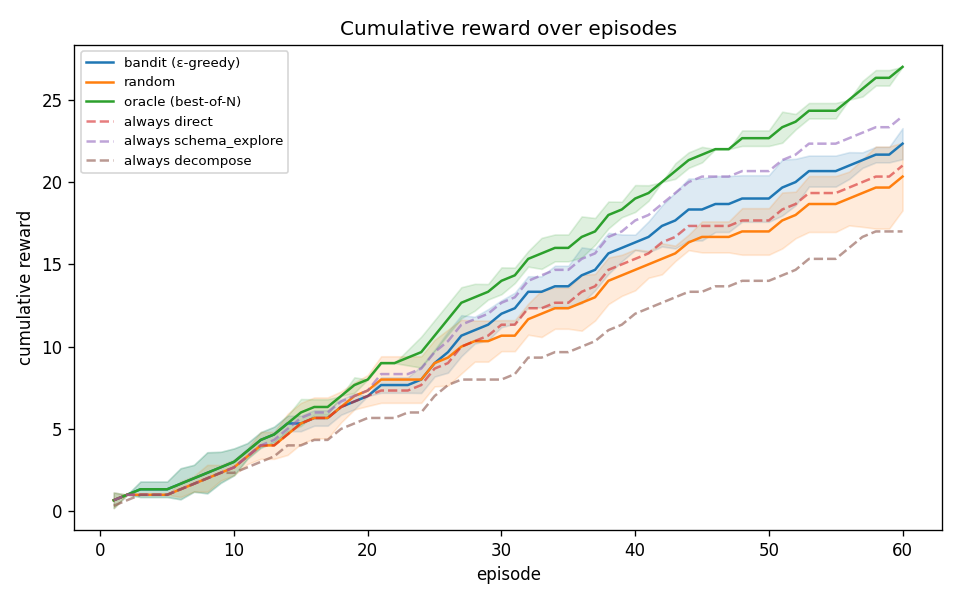
\includegraphics[width=\columnwidth]{exp_01_cumulative_reward.png}
  \caption{Cumulative reward: bandit vs.\ random vs.\ single-arm vs.\ oracle
  (mean $\pm$ std across $3$ seeds). The bandit climbs above random and tracks just
  under the best single arm and the oracle.}
  \label{fig:reward}
\end{figure}

\begin{figure}[t]
  \centering
  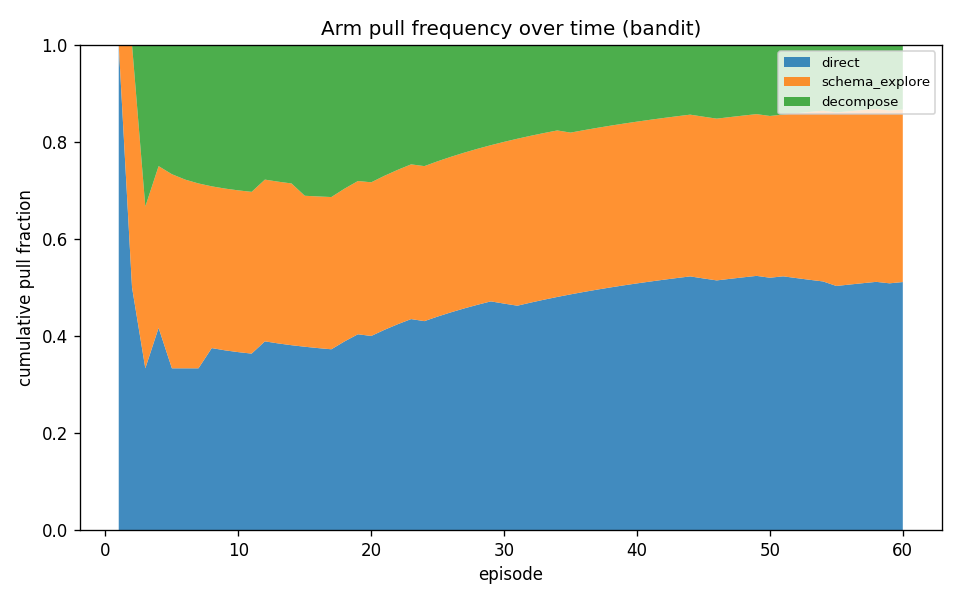
\includegraphics[width=\columnwidth]{exp_02_arm_fractions.png}
  \caption{Arm pull frequency over time. Selection mass moves off the weak
  \code{decompose} arm and onto \code{direct} $+$ \code{schema\_explore}.}
  \label{fig:fractions}
\end{figure}

\begin{figure}[t]
  \centering
  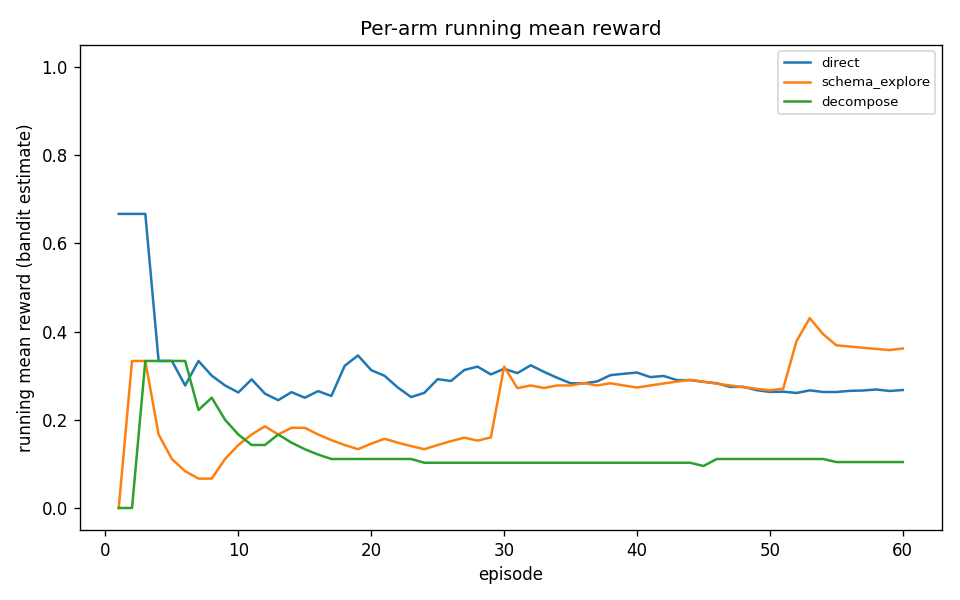
\includegraphics[width=\columnwidth]{exp_04_arm_means.png}
  \caption{Per-arm running mean reward. The bandit's value estimates separate,
  isolating \code{decompose} as the low-value arm.}
  \label{fig:means}
\end{figure}

\textbf{Reading the result honestly.} Because the two strong arms are tied, the
headroom over ``always pick the best arm'' is small. The decisive, reproducible win
is that the bandit learns \emph{online}, without being told the ranking, to avoid the
harmful arm---and lands close to the best fixed policy and the oracle. This is also a
practical lesson the system reports about \emph{itself}: use a selector when your
strategies genuinely differ and you have a cheap signal; when they are tied, the
selector surfaces the tie so you can cut complexity.

\subsection{The selector is domain-agnostic}
The same \code{WorkflowSelector}---no SQL, no BIRD---learns the best arm across three
further domains, each defined only by its arms and a reward
(Table~\ref{tab:domains}). Fig.~\ref{fig:sweep} sweeps policies $\times$ domains and
shows the selector concentrating on the winning arm in every case.

\begin{table}[h]
\centering
\caption{One selector, four domains (arms $+$ reward plugged in).}
\label{tab:domains}
\small
\begin{tabular}{p{1.55cm}p{2.7cm}p{1.45cm}p{0.75cm}}
\toprule
Domain & Arms & Reward & Best \\
\midrule
text-to-SQL (BIRD) & direct / schema-explore / decompose & execution match & schema \\
code gen.\ & direct / iterative-repair / decompose & unit tests pass & iter. \\
agentic search & keyword / iterative / broad$\rightarrow$narrow & file match & iter. \\
compaction$^\dagger$ & truncate / extractive / hierarchical & downstream QA & hier. \\
\bottomrule
\end{tabular}
\\[2pt]
{\footnotesize $^\dagger$Compaction arms adapted from prior coursework
(\textit{ee392c-agent-mem}); we add the downstream-QA reward it lacked.}
\end{table}

\begin{figure}[t]
  \centering
  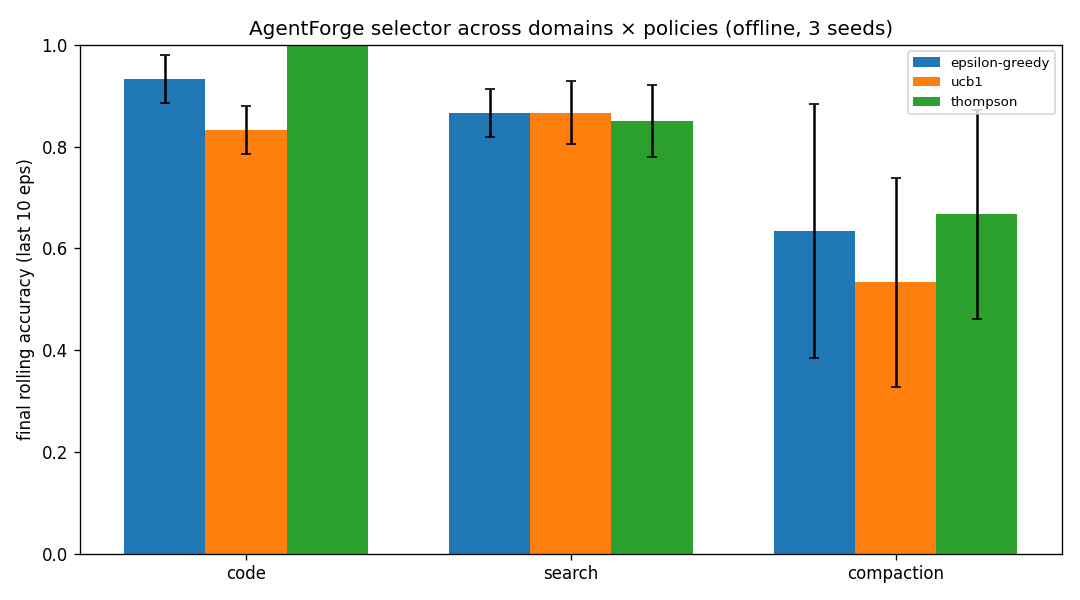
\includegraphics[width=\columnwidth]{sweep_matrix.png}
  \caption{Cross-domain $\times$ policy sweep. The learned selection layer is
  genuinely domain-agnostic: the policy concentrates on the best arm across code,
  search, and compaction as well as SQL.}
  \label{fig:sweep}
\end{figure}

\subsection{Climbing the ladder: contextual and multi-step}
On a synthetic context-dependent task where the best arm \emph{depends on} task
features, the contextual \textbf{LinUCB} policy reaches $1.00$ average reward versus
$\sim$$0.50$ for the context-free bandits, which can only learn the best arm on
average. On the multi-hop ``iterate-or-stop'' environment, the multi-step
\textbf{REINFORCE} controller reaches $0.81$ versus $0.35$ for the best
fixed-horizon policy and $0.19$ for random---a $2.3\times$ improvement over random
(Fig.~\ref{fig:rl}). These two rungs are evaluated on synthetic stand-ins designed to
isolate, respectively, per-task and trajectory-level structure; they demonstrate that
the same kernel extends up the ladder.

\begin{figure}[t]
  \centering
  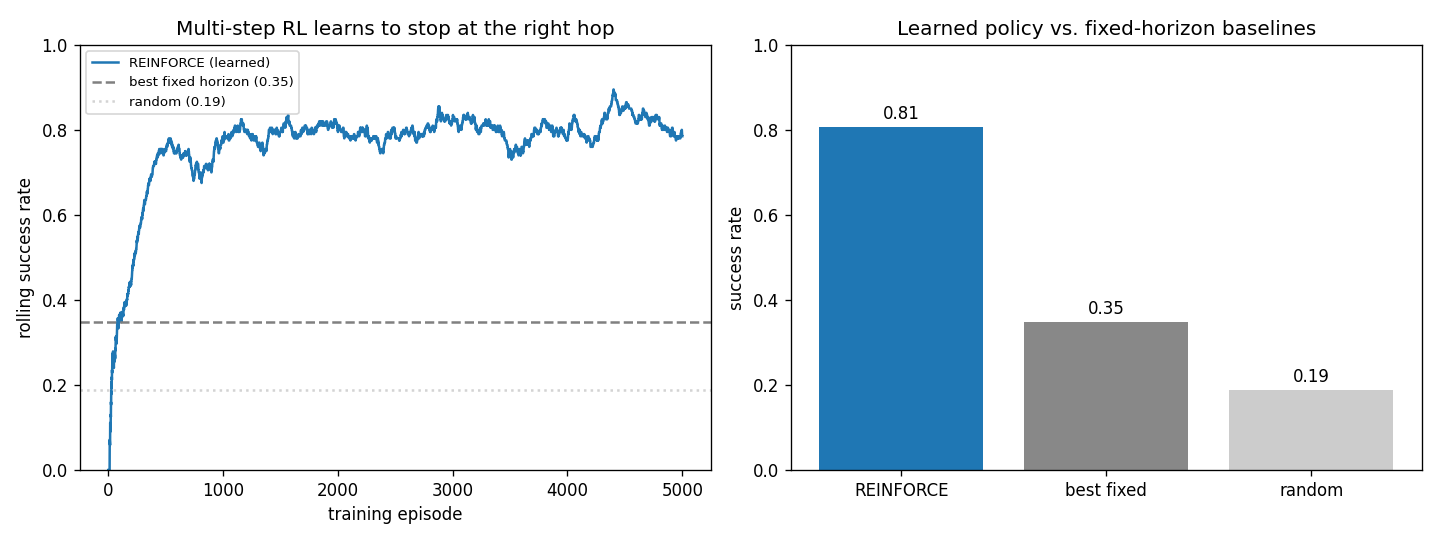
\includegraphics[width=\columnwidth]{rl_multihop.png}
  \caption{Multi-step REINFORCE on the iterate-or-stop environment: the learned
  trajectory-control policy ($0.81$) beats every fixed horizon (best $0.35$) and
  random ($0.19$).}
  \label{fig:rl}
\end{figure}

%------------------------------------------------------------------------------
\section{Limitations}
%------------------------------------------------------------------------------
We state limitations plainly. (i) On BIRD the bandit-vs-random gap is a $3$-seed
mean and the two top arms are statistically tied, so the durable claim is
\emph{online avoidance of the weak arm}, not separating near-identical arms; $60$
episodes is also too short to establish a sub-linear regret \emph{rate}.
(ii) The cross-domain offline demos are \emph{controlled demonstrations}: a scripted
fake LLM makes the arms differ the way real strategies plausibly would, and although
rewards are always computed from each arm's \emph{actual output} (real subprocess
execution, real search, real fact-retention), the fakes have scripted access to
reference answers by design---so they validate \emph{mechanics}, not discovery of
strategy quality in an arbitrary real domain. (iii) The contextual and multi-step
results use synthetic stand-ins. (iv) The code-domain executor is a \emph{toy
harness, not a security sandbox}---untrusted code must not be run through it.
(v) BIRD's gold SQL carries documented label noise, and our white-space positioning
claim is scoped ``to our knowledge (June 2026).''

%------------------------------------------------------------------------------
\section{Conclusion and Future Work}
%------------------------------------------------------------------------------
AgentForge makes workflow \emph{selection} a learnable layer: a domain-agnostic
online selector that, given a few strategies and a cheap reward, concentrates on what
works, drops what doesn't, and persists across runs. It ships the way developer tools
win---open source, a ten-line drop-in, no lock-in---sitting on top of the
orchestration SDK a team already uses. The natural extensions are a cost-adjusted
reward (accuracy per dollar), richer contextual features on real tasks so selection
is per-task rather than on-average, and, longer-term, making the workflows themselves
learnable objects improved from demonstrations, with the selector ranging over an
evolving library.

%------------------------------------------------------------------------------
\section*{Acknowledgment and AI-use disclosure}
%------------------------------------------------------------------------------
Per course policy: this project was implemented with substantial assistance from
\textbf{Claude Code} (Anthropic), which scaffolded the module structure and wrote the
workflow, bandit, executor, reward, logging, and plotting code and tests from the
author's specification. The project design, specification, and all framing decisions
are the author's; AI-generated code was reviewed and verified by the author (offline
test suite $+$ dry run before any API spend). Compaction arms are adapted from the
author's prior coursework (\textit{ee392c-agent-mem}). Developed for Stanford CS\,153
(Frontier Systems), Spring 2026.

\bibliographystyle{IEEEtran}
\bibliography{references}

\end{document}
